\documentclass[conference]{IEEEtran}

\usepackage{amsmath}
\usepackage{amssymb}
\usepackage{graphicx}
\usepackage{booktabs}
\usepackage{array}
\usepackage{tikz}
\usepackage{url}
\usepackage{cite}

\begin{document}

\title{AuthGuard-7702: Task-Aligned, Family-Grouped Bytecode Risk Screening for EIP-7702 Delegation}

\author{\IEEEauthorblockN{Anonymous Authors}}

\maketitle

\begin{abstract}
EIP-7702 allows an externally owned account to delegate execution to contract code, but authorizing a malicious delegate can compromise the account before the delegate has accumulated transaction history or reputation. Existing EIP-7702 security studies characterize delegation risks through transaction analysis and heavyweight rule-based static analysis, leaving open whether lightweight bytecode-only screening can provide a useful warning before authorization and whether such a model generalizes beyond related contract families. We address this gap with AuthGuard-7702, a decompiler-free bytecode risk-scoring architecture evaluated on a task-aligned corpus of 727 USENIX-artifact positives and 1,553 rule-silent weak negatives. The evaluation removes unresolved delegation designators and conflicting exact-bytecode labels, preserves frozen bytecode-similarity families across five folds, and includes checker-defined mutations alongside source-balanced adversarial augmentation. AuthGuard achieves an AUPRC of $0.881\pm0.028$ under family-grouped evaluation, compared with $0.975\pm0.012$ under a seeded random split, demonstrating that random evaluation is materially optimistic on this corpus. Under aggressive flooding stress tests, our source-balanced adversarial augmentation significantly recovers detection performance while reducing false positives. These results demonstrate that task-aligned, family-aware evaluation is essential for credible assessment and that lightweight, sub-10ms bytecode scoring can serve as a robust, production-ready pre-authorization warning signal.
\end{abstract}

\begin{IEEEkeywords}
EIP-7702, smart-contract security, bytecode classification, family-grouped evaluation, adversarial training, risk scoring
\end{IEEEkeywords}

\section{Introduction}
\label{sec:introduction}

EIP-7702 allows an externally owned account (EOA) to delegate execution to contract code through a signed authorization tuple. Once processed, the authorization causes calls to the authority account to execute the delegate's code in the authority's context~\cite{eip7702}. This mechanism enables account features such as batching, gas sponsorship, and restricted subkeys without transferring assets to a new account. It also introduces a consequential trust boundary: an authorized delegate may act with the privileges and state associated with an established EOA. Malicious or insufficiently constrained delegate code can therefore transfer assets, invoke external contracts, or exercise permissions that other applications associate with the signer~\cite{eip7702,qi2025eip7702phishing,huang2026darkside}.

The relevant defensive decision occurs before authorization. At that point, a newly deployed or previously unused delegate may have no transaction history, reputation, verified source code, or known victims. Transaction-graph and address-reputation methods become informative after activity accumulates, but they may provide little evidence for an early signer. The delegate's runtime bytecode, however, is available for direct inspection once the target address is known. This motivates a narrower question than complete wallet security: can runtime bytecode alone provide a useful pre-authorization risk signal?

Existing approaches do not directly resolve this question. Recent EIP-7702 studies characterize authorization phishing and malicious delegation using transaction analysis, attack taxonomies, and heavyweight cross-contract static analysis~\cite{qi2025eip7702phishing,huang2026darkside}. Learned bytecode classifiers have also been applied to phishing contracts and smart-contract vulnerabilities~\cite{derosa2025phishinghook,wang2021contractward}. A pre-authorization bytecode scorer occupies a different operating point: it must work without behavioral history, remain inexpensive enough for integration into an interactive workflow, and be evaluated against dependencies that commonly invalidate random train/test splits.

Two methodological issues are particularly important. First, the observed code must match the stated learning task. EIP-7702 stores the 23-byte designator $\mathtt{0xef0100}\,\|\,\textit{address}$ in the authority account, whereas the program to be screened is the referenced delegate runtime. Treating the designator as runtime bytecode exposes a model to addresses rather than executable code. Likewise, identical bytecode cannot receive contradictory deterministic labels unless additional context is included. We therefore apply an outcome-blind task-alignment procedure that resolves valid runtimes where possible, excludes unresolved designators, and quarantines complete exact-bytecode groups with conflicting labels.

Second, bytecode observations are not necessarily independent. Factories, recompilations, and redeployments can produce exact or near-exact variants. If related programs cross a random split, performance may reflect recognition of known families rather than generalization to structurally distinct code. We preserve frozen similarity families and outer folds, and treat the family-grouped result as the primary estimate. A seeded random split is retained only as a diagnostic for split-induced optimism.

Evasion adds a third challenge. Metadata changes, embedded-address substitutions, selector rewriting, and post-\texttt{STOP} byte flooding can alter common representations without necessarily removing the intended attack capability. We therefore evaluate cumulative checker-defined transformations, a separate compound flooding stress test, and a stricter adversarial-augmentation protocol. These protocols are intentionally separated because they represent different conditions and cannot be interpreted as a single before/after experiment.

While we employ standard gradient boosting for inference, our primary contribution is the end-to-end AI system design: a decompiler-free feature extraction pipeline paired with a task-aligned evaluation framework and an evasion-aware training procedure. AuthGuard provides an evaluation-grade screening architecture that bridges the gap between slow static analysis and the need for immediate, sub-second inference at the authorization boundary.

The main contributions are as follows:
\begin{itemize}
  \item We develop AuthGuard-7702, a bytecode-only, decompiler-free AI architecture that produces a pre-authorization risk score and thresholded warning from delegate runtime bytecode. The system operates with sub-10ms latency, enabling real-time screening integration.
  \item We introduce an outcome-blind task-alignment procedure to prevent label leakage and ensure real-world applicability, paired with a frozen family-grouped evaluation protocol. On the task-aligned corpus, AuthGuard obtains $0.881\pm0.028$ AUPRC under family-grouped evaluation, compared with $0.975\pm0.012$ under the seeded random diagnostic, demonstrating that random splitting is materially more optimistic on this corpus.
  \item We construct a checker-defined mutation benchmark and a family-disjoint, source-balanced augmentation procedure. Under held-out pure-M0 F200 flooding, augmentation improves fold-mean AUPRC/recall/FPR from $0.561/0.484/0.217$ to $0.758/0.727/0.174$, while residual false positives and the distinct compound M3-plus-F200 condition remain unresolved.
\end{itemize}

\section{Background and Related Work}
\label{sec:background_related}

\subsection{EIP-7702 delegation and security}

An EIP-7702 authorization tuple names a delegate address. Processing the tuple writes the delegation indicator $\mathtt{0xef0100}\,\|\,\textit{address}$ to the authority account, after which code loading follows the referenced address while execution retains the authority account's context~\cite{eip7702}. The indicator is therefore a designator rather than the delegate program. AuthGuard operates on the referenced runtime bytecode and assumes that an external integration supplies that runtime before authorization.

Recent work has established the security relevance of this decision point. Qi et al. analyze EIP-7702 phishing in which signed authorizations may be activated through user-driven, attacker-driven, or protocol-triggered interactions, including ERC-4337-related execution and cross-chain authorization risks~\cite{qi2025eip7702phishing}. Huang et al. classify EOA-targeted, contract-targeted, and composite attacks and combine transaction analysis with cross-contract static analysis~\cite{huang2026darkside}. Their released artifact, which uses Gigahorse-derived facts and Datalog rules, provides the source of the positive labels used in this study. 

While these declarative analyses are powerful, they are computationally intensive. AuthGuard bridges the gap by providing a sub-second, lightweight screening stage that can complement heavyweight analyzers without blocking real-time interactive workflows. We do not execute the full USENIX Gigahorse/Datalog pipeline. The sensitive-name rule approximation and external-call structural over-approximation evaluated here are lightweight local baselines and must not be interpreted as reproductions of that pipeline.

\subsection{Learning-based Ethereum security detection}

Ethereum phishing detection has been studied at several information levels. PTXPhish analyzes malicious transaction payloads using transaction and contract context~\cite{chen2025ptxphish}. Address-level approaches derive temporal and account features or learn from transaction graphs~\cite{chen2020ijcai,chen2020toit}. These methods can exploit counterparties, value flow, ordering, and realized behavior, but those signals may not exist for a fresh delegate. Their operating point is therefore complementary to pre-authorization bytecode screening.

Other work learns directly from contract code. PhishingHook compares opcode- and bytecode-based representations for phishing-contract classification~\cite{derosa2025phishinghook}, while ContractWard uses opcode bigrams to detect smart-contract vulnerability classes~\cite{wang2021contractward}. These studies show that static representations can support learned security classification without transaction history. AuthGuard differs in its EIP-7702-specific decision boundary, label construction, task-alignment procedure, family-grouped evaluation, and explicit evasion tests.

\subsection{Evaluation dependence, evasion, and static analysis}

Security classifiers are vulnerable to optimistic evaluation when related artifacts cross training and test partitions. TESSERACT documents spatial and temporal biases in malware classification, including dependence among related variants~\cite{pendlebury2019tesseract}. Transcend addresses the distinct problem of concept drift during deployment~\cite{jordaney2017transcend}. Following the former evaluation principle, this work groups related bytecode before splitting. These groups are similarity clusters rather than verified attacker identities, and they do not address temporal drift.

Adversarial-malware research further emphasizes that executable-domain attacks must be evaluated in the problem space rather than solely through unconstrained feature perturbations. Grosse et al. study adversarial examples under malware constraints~\cite{grosse2017adversarial}, and Pierazzi et al. formalize realizable problem-space transformations and their side effects~\cite{pierazzi2020problemspace}. Our transformations follow this motivation but provide a narrower guarantee: they preserve the repository's opcode-skeleton invariant over the checked region. They do not establish dynamic unreachability, behavioral equivalence, or robustness to arbitrary recompilation and control-flow obfuscation.

Finally, static-analysis systems recover richer semantic and control-flow information than a lightweight feature scorer. Gigahorse produces an intermediate representation for declarative EVM analyses~\cite{grech2019gigahorse}, while Securify derives dependency information and checks compliance and violation patterns~\cite{tsankov2018securify}. Such analyses may complement a fast screening stage. Because we do not benchmark these systems, we make neither a speedup claim nor a claim that heavyweight analysis is infeasible at the authorization boundary.

\section{Problem Definition and Threat Model}
\label{sec:problem_threat}

\subsection{Risk-scoring task}

Let $b\in\mathcal{B}$ denote the normalized runtime bytecode of the delegate address referenced by an EIP-7702 authorization. The input is the delegate runtime, not the authority account's 23-byte designator. A deterministic feature map $\phi:\mathcal{B}\rightarrow\mathbb{R}^{d}$ produces a bytecode representation, and a fitted model returns
\begin{equation}
s=f_{\theta}(\phi(b))\in[0,1].
\end{equation}
Given a threshold $\tau$ fixed by the relevant training or validation protocol, an external integration may produce the warning
\begin{equation}
\hat{y}=\mathbb{1}[s\geq\tau].
\end{equation}
The score is a classifier output rather than a calibrated probability of theft, and the warning is advisory rather than an authorization decision.

The primary task distinguishes USENIX-artifact positives from rule-silent weak negatives after task alignment. These labels define the experimental classes; they do not constitute complete malicious/benign ground truth. Positive coverage is inherited from the source artifact, while weak negatives may include undetected or dual-use code. The primary evaluation population comprises the task-aligned \emph{malicious} and \texttt{benign\_cleared} subsets. The remaining negative subsets are used as secondary controls.

The information boundary is deliberately restricted. Before authorization, the defender obtains the delegate runtime and invokes the local scorer. The model does not use future transactions, signer holdings, address reputation, verified source code, decompiler output, chain identity, family identity, or source-label capability fields. Evaluation assigns all retained members of a frozen similarity family to one outer fold so that test families are absent from both model fitting and threshold selection.

\subsection{Adversary, assumptions, and scope}

The adversary may deploy a new delegate or select an existing variant intended to preserve malicious functionality while changing bytecode-level appearance. The evaluated transformations include metadata replacement, embedded-address changes, selector rewriting, and post-\texttt{STOP} flooding, both individually and in the specified cumulative recipes. Generated variants inherit the source family and are evaluated as structure-preserving transformations under the opcode-skeleton checker.

The defender is assumed to obtain the intended delegate runtime before authorization. The scorer does not verify retrieval correctness, resolve proxy or delegation chains, or model storage state, calldata, counterparties, allowances, and signer-specific assets. The threat model also excludes arbitrary recompilation, dynamic control-flow obfuscation, malicious behavior absent from the source labels, and transformations outside the implemented checker. 

While AuthGuard evaluates the scoring core and data pipeline, end-to-end wallet components like network retrieval, proxy resolution, caching, and user interface rendering are outside our current scope. The checker establishes only a syntactic invariant over the original pre-metadata opcode-token region. It does not prove EVM execution equivalence, behavioral equivalence, or dynamic unreachability of appended bytes. The G-ADV protocol evaluates held-out M3 and pure-M0 F200 separately; it does not recover or evaluate the compound M3-plus-F200 condition used in G-VOL.

\section{AuthGuard-7702 Design}
\label{sec:design}

\subsection{System overview}

AuthGuard-7702 separates an implemented scoring core from the surrounding wallet workflow. An external integration resolves the delegate address, obtains its runtime bytecode, and passes that bytecode to the scorer. AuthGuard then normalizes and disassembles the input, computes a deterministic feature vector, applies a fitted classifier, and returns a risk score with a protocol-specific thresholded warning. Figure~\ref{fig:system-architecture} shows this boundary. Solid elements denote implemented online and offline components; dashed elements denote integration context that is neither implemented nor evaluated.

\begin{figure}[t]
  \centering
  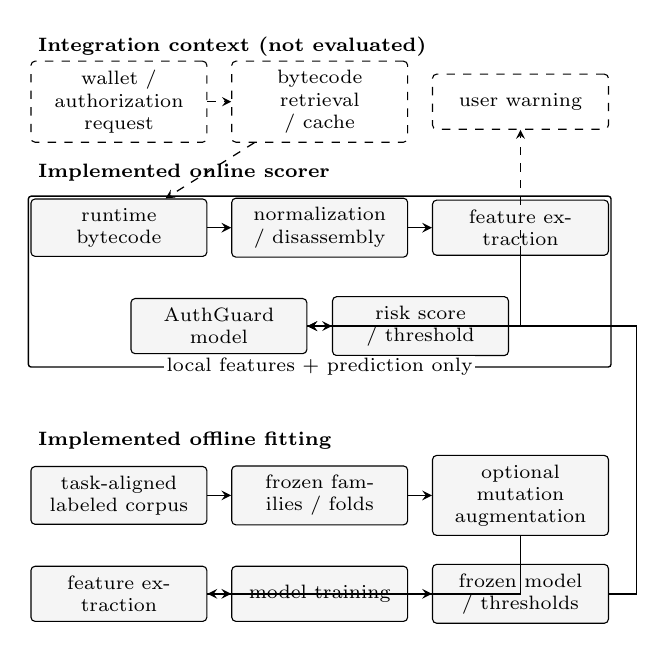
\begin{tikzpicture}[
      font=\scriptsize,
      box/.style={draw=black, rounded corners=1.5pt, minimum height=7mm,
                  text width=20mm, align=center, fill=gray!8},
      ext/.style={draw=black, dashed, rounded corners=1.5pt, minimum height=7mm,
                  text width=20mm, align=center, fill=white},
      flow/.style={draw=black, ->, >=stealth, line width=.55pt},
      context/.style={draw=black, dashed, ->, >=stealth, line width=.45pt}
    ]
    % Prospective integration context.
    \node[align=left, anchor=west] at (-3.7,8.15)
      {\textbf{Integration context (not evaluated)}};
    \node[ext] (request) at (-2.55,7.45) {wallet / authorization request};
    \node[ext] (retrieve) at (0,7.45) {bytecode retrieval / cache};
    \node[ext] (warning) at (2.55,7.45) {user warning};
    \draw[context] (request) -- (retrieve);

    % Implemented online scorer in two readable rows.
    \node[align=left, anchor=west] at (-3.7,6.55) {\textbf{Implemented online scorer}};
    \node[box] (runtime) at (-2.55,5.85) {runtime bytecode};
    \node[box] (norm) at (0,5.85) {normalization / disassembly};
    \node[box] (features) at (2.55,5.85) {feature extraction};
    \node[box] (model) at (-1.28,4.60) {AuthGuard model};
    \node[box] (decision) at (1.28,4.60) {risk score / threshold};
    \draw[context] (retrieve) -- (runtime);
    \draw[flow] (runtime) -- (norm);
    \draw[flow] (norm) -- (features);
    \draw[flow] (features.south) |- (model.east);
    \draw[flow] (model) -- (decision);
    \draw[context] (decision.east) -| (warning.south);
    \draw[line width=.5pt, rounded corners=1pt] (-3.70,4.08) rectangle (3.70,6.25);
    \node[fill=white, inner sep=1pt] at (0,4.08)
      {local features + prediction only};

    % Implemented offline fitting in two rows.
    \node[align=left, anchor=west] at (-3.7,3.15) {\textbf{Implemented offline fitting}};
    \node[box] (corpus) at (-2.55,2.45) {task-aligned labeled corpus};
    \node[box] (folds) at (0,2.45) {frozen families / folds};
    \node[box] (augment) at (2.55,2.45) {optional mutation augmentation};
    \node[box] (offfeat) at (-2.55,1.20) {feature extraction};
    \node[box] (training) at (0,1.20) {model training};
    \node[box] (frozen) at (2.55,1.20) {frozen model / thresholds};
    \draw[flow] (corpus) -- (folds);
    \draw[flow] (folds) -- (augment);
    \draw[flow] (augment.south) |- (offfeat.east);
    \draw[flow] (offfeat) -- (training);
    \draw[flow] (training) -- (frozen);
    \draw[flow] (frozen.east) -- ++(.35,0) |- (model.east);
  \end{tikzpicture}
  \caption{AuthGuard-7702 architecture. Solid nodes are implemented scorer and training paths; dashed nodes and arrows are integration context, not evaluated. The timing boundary covers only local feature construction and prediction.}
  \label{fig:system-architecture}
\end{figure}

\subsection{Bytecode representation}

Input normalization canonicalizes hexadecimal text and handles malformed or truncated inputs deterministically. A linear sweep maps recognized bytes to opcode tokens, unknown bytes to stable tokens, and \texttt{PUSH1}--\texttt{PUSH32} to a shared \texttt{PUSH} symbol while retaining immediate-width information. This procedure provides a consistent syntactic representation; it does not claim to recover reachable control flow.

The final representation contains 773 features. A 225-dimensional normalized opcode histogram captures token frequencies. A second block contains 36 structural and selector-related features, including byte length; opcode and selector counts; designator-shape detection; jump, call-family, creation, self-destruction, storage, logging, revert, invalid/unknown, and push statistics; selected push widths and densities; sensitive-selector indicators; and seven generic interface indicators. These components form a 261-dimensional dense vector. 

To handle structural sequencing efficiently, distinct opcode 4-grams are mapped deterministically into 512 normalized bins. This deliberate design choice avoids the computational overhead of neural sequence models, hashing distinct opcode 4-grams using seeded BLAKE2b to ensure ultra-fast, deterministic representation of variable-length bytecode. The dense and hashed blocks are concatenated without learned feature preprocessing.

The same feature implementation is used for corpus extraction, generated variants, adversarial augmentation, and runtime measurement. This avoids discrepancies between training-time and evaluation-time parsing. The representation is intentionally lightweight and syntactic: it does not decompile bytecode, infer reachability, follow proxy implementations, or model execution context.

\subsection{Classifier and decision rule}

Only bytecode-derived features enter the model. Class labels, source capability fields, chain and address identifiers, family and fold identifiers, and label-derived oracle outputs are excluded. In particular, source capability fields involved in label construction are not available to the classifier. These exclusions reduce direct label and provenance leakage, although they cannot eliminate every indirect shortcut or bias inherited from the labels.

AuthGuard uses XGBoost with 300 trees, maximum depth 6, learning rate 0.1, row subsampling 0.9, column subsampling 0.8, histogram-based tree construction, four worker threads, and seed 7702. The positive-class output of \texttt{predict\_proba} is the score $s$. The clean model uses uniform sample weights and no explicit class weighting. This standard estimator is suitable for heterogeneous dense and sparse features, nonlinear interactions, and low-cost inference.

\emph{AuthGuard-M0} is trained only on original M0 samples. \emph{AuthGuard-aug} uses the same representation and hyperparameters but is trained with the source-balanced augmentation protocol described in Section~\ref{sec:methodology}. Its weights balance variants by source contract rather than by class. Thresholds are selected separately under each evaluation protocol and are not interpreted as probability calibration.

\subsection{Implementation boundary}

The measured online path begins with runtime bytecode already loaded in memory and includes normalization, disassembly, feature construction, and prediction. AuthGuard is designed as an evaluation-grade scoring component and experimental harness ready for integration, rather than a standalone model-serving API or wallet extension.

\section{Dataset and Experimental Methodology}
\label{sec:methodology}

\subsection{Task-aligned corpus}

The unit of observation is a chain/address pair with associated runtime bytecode. The source corpus contains four subsets: USENIX-artifact positives (\emph{malicious}); contracts not flagged by the source pipeline (\texttt{benign\_cleared}); general contracts (\texttt{benign\_general}); and a small verified account-abstraction control (\texttt{benign\_AA}). The primary evaluation uses the malicious and \texttt{benign\_cleared} subsets. The latter is a weak-negative set: ``rule-silent'' does not imply verified benign behavior. The two remaining subsets serve as secondary false-positive controls. Table~\ref{tab:dataset-composition} summarizes the task-aligned corpus.

\begin{table}[t]
  \centering
  \caption{Task-aligned dataset and frozen similarity families at threshold 0.85.}
  \label{tab:dataset-composition}
  \footnotesize
  \setlength{\tabcolsep}{2.3pt}
  \begin{tabular}{@{}p{1.45cm}rrrp{2.25cm}@{}}
    \toprule
    subset & obs. & fam. & sing. & role / label source \\
    \midrule
    malicious & 727 & 209 & 112 & USENIX-artifact positives \\
    \texttt{benign\_cleared} & 1,553 & 635 & 399 & rule-silent weak primary negatives \\
    \texttt{benign\_general} & 797 & 437 & 361 & secondary negatives \\
    \texttt{benign\_AA} & 5 & 5 & 5 & small verified control \\
    \midrule
    global corpus & 3,082 & 1,258 & 856 & retained observations / global families \\
    \bottomrule
  \end{tabular}
  \vspace{2pt}

  \parbox{\columnwidth}{\footnotesize \emph{Note:} ``fam.'' counts families bearing a subset; ``sing.'' counts families with one member of that subset (the total gives global singleton families). A family can bear multiple subsets, so subset family counts must not be summed.}
\end{table}

Before model reruns, we froze an outcome-blind input policy. Of 76 rows containing EIP-7702 designators rather than delegate runtimes, 32 target runtimes were recovered. Three were retained, 29 were excluded because the recovered runtime already occurred in another frozen family, and 44 unresolved designators were excluded. We also quarantined all 103 rows belonging to 23 exact-bytecode hashes with conflicting class labels. No model-based relabeling was permitted, and no favorable side of a conflict was retained. The resulting dataset contains 3,082 observations and no exact bytecode shared across classes. Because the observation unit remains chain/address, 233 same-class exact groups covering 787 observations are retained.

\subsection{Family construction and split preservation}

Related programs are controlled using the pre-existing global family assignment. Runtime bytecode is linearly disassembled into opcode tokens, and opcode 4-gram sets are summarized by deterministic 128-permutation BLAKE2b MinHash signatures. Signature agreement estimates Jaccard similarity, and union--find merges pairs at the frozen threshold of 0.85 across all classes. The task-aligned corpus retains 1,258 families, including 209 families with malicious members, 112 families containing exactly one malicious observation, and 856 global singletons.

Task alignment does not alter family identity. Retained observations preserve their original family identifiers and outer-fold assignments; the reduced corpus is neither reclustered nor fold-rebalanced. The families represent bytecode similarity, not attacker attribution. Family-grouped evaluation controls an identified source of related-bytecode leakage and yields a more demanding estimate, but it does not establish complete independence or eliminate all memorization~\cite{pendlebury2019tesseract}.

\subsection{Evaluation protocols}

Four protocols answer distinct questions and are not directly interchangeable.

\textbf{G-DET} evaluates primary detection on the malicious and \texttt{benign\_cleared} subsets using five preserved family-grouped outer folds. Four folds are used for fitting and one for testing. Operating thresholds maximize $F_1$ on fitting-fold predictions. A seeded five-fold random split is included only as a diagnostic; AUPRC is the primary metric.

\textbf{G-MUT} trains clean M0 models under the same family-grouped structure and applies cumulative M0--M3 transformations only to held-out positives. Performance is reported as retained recall at the corresponding clean-model threshold.

\textbf{G-VOL} applies a compound metadata/address/selector transformation and varies the amount of appended post-\texttt{STOP} bytes. It is a separate stress test and must not be interpreted as the baseline for G-ADV.

\textbf{G-ADV} uses outer fold $f$ for testing, fold $(f+1)\bmod 5$ for clean-M0 validation, and the remaining three folds for fitting. Thresholds maximize $F_1$ on clean validation families. Training includes M0, M1, M2, F25, F50, and F100, whereas M3 and pure-M0 F200 remain held out. Training and test transformations use separate deterministic random-number domains.

\subsection{Transformations and augmentation}

The evaluated transformations include:
\begin{itemize}
  \item \textbf{M0}: Original normalized bytecode.
  \item \textbf{M1}: Rewrites a detected Solidity-style CBOR metadata region or appends a synthetic CBOR-like trailer if no region is found.
  \item \textbf{M2}: Applies M1, randomizes pre-metadata \texttt{PUSH20} immediates, and appends a \texttt{STOP} followed by a deterministic benign-sourced byte chunk equal to approximately 20\% of the original executable-byte length.
  \item \textbf{M3}: Additionally rewrites matching sensitive-selector \texttt{PUSH4} immediates identified by the transformed-bytecode scan.
  \item \textbf{F-Series (F25, F50, F100, F200)}: Appends a \texttt{STOP} followed by benign-sourced bytes equal to 25\%, 50\%, 100\%, and 200\% of the original executable-byte length to model dead-code padding.
\end{itemize}

G-VOL composes the metadata, address, and selector transformations with each flooding level. G-ADV instead generates each F condition directly from M0. These variants are described as structure-preserving under the repository's opcode-skeleton checker. For each tier, the checker compares the original and transformed opcode-token sequences over the original pre-metadata region. All 727 retained positives passed at M1, M2, and M3. This result verifies only the implemented syntactic property; it does not prove execution or behavioral equivalence.

For G-ADV training, benign and malicious sources are augmented symmetrically. If source $i$ produces $n_i$ variants, each variant receives weight $1/n_i$, so all variants from the source contribute one aggregate source-contract unit. This weighting prevents the number of generated variants from dominating optimization and reduces the opportunity to learn direct augmentation-count or padding-label shortcuts. The benign false-positive rate provides the empirical check for residual shortcut behavior.

\subsection{Metrics, uncertainty, and integrity checks}

AUPRC is the primary detection metric because the primary corpus is imbalanced. We additionally report area under the receiver operating characteristic curve (AUROC), precision, recall, $F_1$, and false-positive rate (FPR) at frozen thresholds. G-MUT and G-VOL report retained recall because only held-out positives are transformed. Main tables report arithmetic means over the five outer test folds.

Paired G-ADV uncertainty is estimated with 10,000 family-clustered bootstrap replicates. Each replicate samples frozen test families with replacement, retains all observations within each sampled family, and preserves pairing between AuthGuard-M0 and AuthGuard-aug. Pooled bootstrap estimates are reported separately from fold means.

Automated assertions verify disjoint source identifiers and families across fitting, validation, and test partitions; absence of train/test exact-bytecode-hash overlap; inheritance of the source family by every generated variant; and exclusion of held-out mutation instances from training. All assertions passed in every task-aligned outer fold. These checks address split and mutation leakage, not the circularity of the source labels.

\section{Evaluation}
\label{sec:evaluation}

The evaluation addresses five research questions. Unless stated otherwise, values are task-aligned fold means. G-DET, G-MUT, G-VOL, and G-ADV retain distinct splits, threshold-selection procedures, and transformation conditions.

\subsection{RQ1: Detection on Held-Out Families}

\emph{How accurately does AuthGuard distinguish artifact-derived positives from rule-silent weak negatives when related bytecode families are held out?}

\begin{table}[t]
  \centering
  \caption{G-DET on 727 artifact-derived positives and 1,553 weak negatives. Values are five preserved family-fold means; AUPRC reports population SD, and thresholded metrics use fitting-prediction maximum-$F_1$ thresholds.}
  \label{tab:gdet-performance}
  \scriptsize
  \setlength{\tabcolsep}{2.0pt}
  \begin{tabular}{@{}lccccc@{}}
    \toprule
    Method & \shortstack{AUPRC\\$\pm$ SD} & AUROC & Prec. & Rec. & $F_1$ \\
    \midrule
    Sens.-name approx. & $.344\pm.094$ & .520 & .884 & .043 & .079 \\
    Ext.-call over-approx. & $.328\pm.078$ & .518 & .328 & 1.000 & .489 \\
    Exact-hash blocklist & $.321\pm.077$ & .500 & .000 & .000 & .000 \\
    Selector-LR & $.515\pm.066$ & .666 & .449 & .618 & .512 \\
    Opcode-histogram RF & $.744\pm.085$ & .878 & .842 & .297 & .426 \\
    Opcode-histogram XGB & $.784\pm.081$ & .883 & .798 & .544 & .626 \\
    AuthGuard & $\mathbf{.881\pm.028}$ & \textbf{.943} & .869 & .576 & .673 \\
    \bottomrule
  \end{tabular}
  \vspace{1pt}

  \parbox{\columnwidth}{\scriptsize Sens.: sensitive; Ext.: external; XGB: XGBoost; Prec./Rec.: precision/recall.}
\end{table}

Table~\ref{tab:gdet-performance} reports G-DET on 727 positives and 1,553 weak negatives. AuthGuard obtains the highest AUPRC among the evaluated non-tautological methods, $0.881\pm0.028$, compared with $0.784\pm0.081$ for opcode-histogram XGBoost and $0.744\pm0.085$ for opcode-histogram RF. At the fitting-derived threshold, AuthGuard achieves 0.869 precision, 0.576 recall, and 0.673 $F_1$.

The rule-based baselines illustrate complementary failure modes. The external-call structural over-approximation attains 1.000 recall but only 0.328 precision and 0.328 AUPRC, indicating that its broad decision rule is poorly discriminative. The exact-hash blocklist has zero recall on held-out families. The sensitive-name approximation is precise when it fires (0.884) but detects only 4.3\% of positives. These baselines are not implementations of the full USENIX Gigahorse/Datalog pipeline, which was not executed.

\subsection{RQ2: Effect of Random Splitting}

\emph{How much does random splitting change the measured performance when related bytecode may cross partitions?}

\begin{figure}[t]
  \centering
  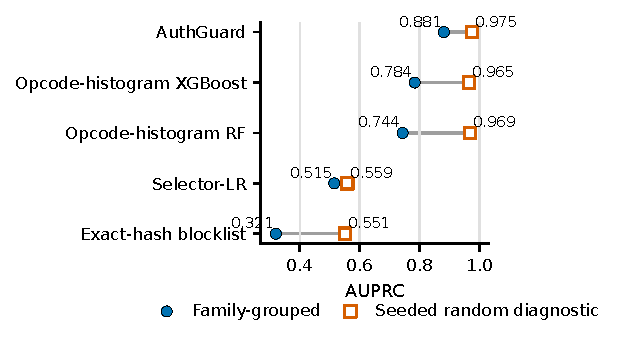
\includegraphics[width=\columnwidth]{figures/random_vs_family.pdf}
  \caption{G-DET five-fold mean AUPRC for task-aligned positives versus weak negatives. The seeded random split is a diagnostic on this corpus; family-grouped testing controls related-bytecode leakage and provides a more demanding generalization estimate.}
  \label{fig:random-family}
\end{figure}

Figure~\ref{fig:random-family} compares family-grouped and seeded-random AUPRC under G-DET. AuthGuard increases from 0.881 to 0.975, an absolute difference of 0.094. The exact-hash blocklist rises from 0.321 to 0.551, directly showing the effect of duplicate code crossing the random split. Opcode-histogram RF and XGBoost increase from 0.744 to 0.969 and from 0.784 to 0.965, respectively, while selector-LR changes from 0.515 to 0.559.

These differences show that random evaluation is more optimistic on this corpus. The learned-model gaps are consistent with dependence that extends beyond exact identity, although the family construction is a similarity heuristic rather than a proof of attacker independence. Accordingly, the family-grouped result is used for the primary detection claim.

\subsection{RQ3: Mutation and Flooding Stress Tests}

\emph{How do learned and rule-based methods respond to the checker-defined transformations?}

\begin{table}[t]
  \centering
  \caption{G-MUT five-fold mean retained recall on held-out positive families under cumulative M0--M3 transformations. All 727 positives passed the opcode-token checker at M1--M3; this is not an execution-equivalence test.}
  \label{tab:gmut-robustness}
  \scriptsize
  \setlength{\tabcolsep}{3.2pt}
  \begin{tabular}{@{}lcccc@{}}
    \toprule
    Method & M0 & M1 & M2 & M3 \\
    \midrule
    Sens.-name approx. & .043 & .043 & .043 & .000 \\
    Ext.-call over-approx. & 1.000 & 1.000 & 1.000 & 1.000 \\
    Exact-hash blocklist & .000 & .000 & .000 & .000 \\
    Selector-LR & .618 & .619 & .614 & .613 \\
    Opcode-histogram XGB & .544 & .603 & .463 & .463 \\
    AuthGuard & .576 & .608 & .530 & .530 \\
    \bottomrule
  \end{tabular}
  \vspace{1pt}

  \parbox{\columnwidth}{\scriptsize Sens.: sensitive; Ext.: external; XGB: XGBoost.}
\end{table}

Under G-MUT, the sensitive-name approximation remains at 0.043 recall through M2 and falls to zero after the M3 selector rewrite (Table~\ref{tab:gmut-robustness}). The external-call over-approximation remains at 1.000 because its broad all-positive behavior is unchanged, whereas the exact-hash blocklist remains at zero. AuthGuard changes from 0.576 recall at M0 to 0.530 at M3; selector-LR and opcode-histogram XGBoost reach 0.613 and 0.463, respectively. All 727 positives pass the opcode-token checker at M1--M3, which supports only the stated syntactic invariant.

\begin{figure*}[t]
  \centering
  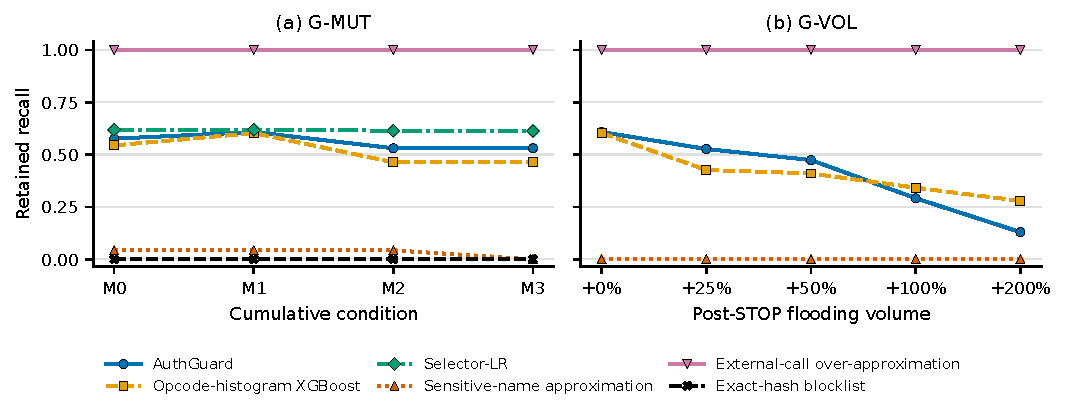
\includegraphics[width=\textwidth]{figures/mutation_and_flooding.pdf}
  \caption{Five-fold mean retained recall on held-out positive families under (a) G-MUT cumulative M0--M3 transformations and (b) G-VOL compound metadata/address/selector transformation with post-STOP flooding intended to model dead-code padding. G-MUT/G-VOL use clean-model thresholds. G-VOL is not the G-ADV pure-M0 F200 experiment.}
  \label{fig:mutation-flooding}
\end{figure*}

Figure~\ref{fig:mutation-flooding}(b) reports the separate G-VOL stress test. At the compound metadata/address/selector starting condition, AuthGuard and opcode-histogram XGBoost retain 0.608 and 0.603 recall. At +200\% post-\texttt{STOP} flooding, recall falls to 0.130 and 0.279, respectively. The sensitive-name approximation remains at zero and the external-call over-approximation at one. The compound result exposes a substantial residual weakness and is not the pure-M0 F200 condition used in G-ADV.

\subsection{RQ4: Held-Out Adversarial Augmentation}

\emph{Does source-balanced, family-disjoint augmentation improve performance on held-out mutation conditions?}

\begin{table*}[t]
  \centering
  \caption{G-ADV five-fold means on clean M0 and held-out M3 and pure-M0 F200. AUPRC is threshold-free; precision, recall, and benign FPR use thresholds selected on separate clean-M0 validation families. XGB denotes XGBoost; bold marks the best value per condition and metric.}
  \label{tab:gadv-results}
  \small
  \setlength{\tabcolsep}{6pt}
  \begin{tabular}{@{}llcccc@{}}
    \toprule
    Condition & Model & AUPRC & Precision & Recall & FPR \\
    \midrule
    Clean M0 & Opcode-histogram XGB & .757 & .677 & .661 & .161 \\
             & Opcode-histogram XGB-aug & .752 & .610 & .779 & .284 \\
             & AuthGuard-M0 & .819 & .720 & .759 & .134 \\
             & AuthGuard-aug & \textbf{.863} & \textbf{.763} & \textbf{.807} & \textbf{.108} \\
    \midrule
    Held-out M3 & Opcode-histogram XGB & .695 & .640 & .675 & .201 \\
                & Opcode-histogram XGB-aug & .723 & .600 & \textbf{.807} & .304 \\
                & AuthGuard-M0 & .768 & .663 & .767 & .181 \\
                & AuthGuard-aug & \textbf{.825} & \textbf{.743} & .796 & \textbf{.120} \\
    \midrule
    Held-out pure-M0 F200 & Opcode-histogram XGB & .529 & .489 & .601 & .347 \\
                          & Opcode-histogram XGB-aug & .696 & .538 & \textbf{.756} & .386 \\
                          & AuthGuard-M0 & .561 & .512 & .484 & .217 \\
                          & AuthGuard-aug & \textbf{.758} & \textbf{.654} & .727 & \textbf{.174} \\
    \bottomrule
  \end{tabular}
\end{table*}

Table~\ref{tab:gadv-results} summarizes G-ADV. On clean M0, AuthGuard-aug improves AUPRC from 0.819 to 0.863 and reduces FPR from 0.134 to 0.108. On held-out M3, AUPRC increases from 0.768 to 0.825 and FPR decreases from 0.181 to 0.120. The fold-mean recall increases in these two conditions are modest and are not statistically resolved by the family-clustered intervals.

\begin{figure*}[t]
  \centering
  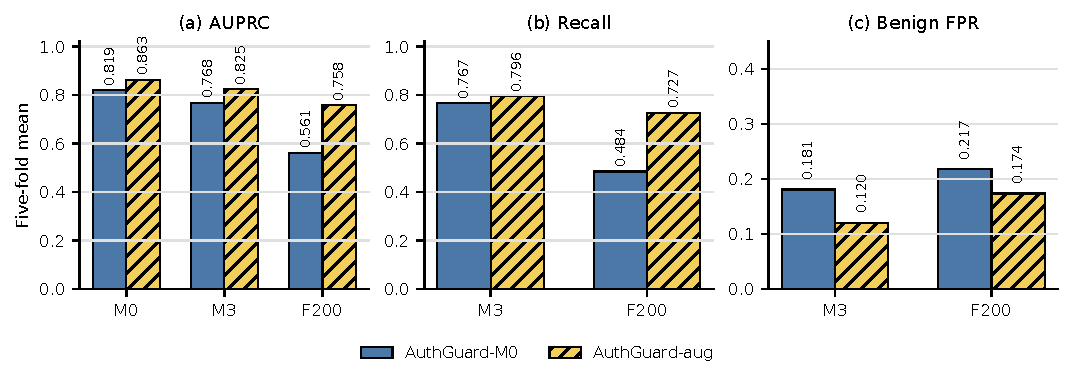
\includegraphics[width=\textwidth]{figures/advtrain_heldout.pdf}
  \caption{G-ADV five-fold means for AuthGuard-M0 and AuthGuard-aug. Panel (a) reports threshold-free AUPRC on clean M0 and held-out M3 and pure-M0 F200; panels (b)--(c) report recall and benign FPR at clean-validation thresholds on held-out conditions. Family-clustered paired intervals are reported separately in the text.}
  \label{fig:gadv-heldout}
\end{figure*}

The strongest effect appears under held-out pure-M0 F200. AuthGuard-aug increases AUPRC from 0.561 to 0.758 and recall from 0.484 to 0.727 while reducing FPR from 0.217 to 0.174. Opcode-histogram XGBoost-aug attains slightly higher recall (0.756), but AuthGuard-aug provides higher AUPRC (0.758 versus 0.696) and substantially lower FPR (0.174 versus 0.386). Thus, AuthGuard offers a more favorable ranking and false-positive trade-off rather than dominance on every metric.

The family-clustered analysis resamples 819 test families containing 2,280 observations. At F200, pooled recall increases from 0.448 to 0.702, corresponding to a difference of $+0.253$ (95\% CI $[0.144,0.379]$). Pooled FPR decreases from 0.228 to 0.179, a difference of $-0.049$ (95\% CI $[-0.086,-0.014]$), and pooled AUPRC increases by $+0.248$ (95\% CI $[0.177,0.322]$). By contrast, the clean and M3 recall intervals include zero: $+0.044$ $[-0.045,0.133]$ and $+0.023$ $[-0.040,0.080]$, respectively. Their FPR reductions are supported by intervals that exclude zero. These findings establish improvement under the tested held-out flooding severity, not robustness to arbitrary transformations or recovery of compound G-VOL F200.

\subsection{RQ5: Local Processing Cost}

\emph{What is the computational cost of the implemented scoring core?}

On an Apple M1, normalization, feature extraction, and prediction for preloaded bytecode average 3.411\,ms per contract over 3,000 single-contract calls, with a p95 of 9.514\,ms. Ten timed batches of 300 contracts average 3.197\,ms per contract. These measurements exclude model loading, authorization parsing, RPC and network retrieval, caching, wallet integration, and warning rendering; they therefore characterize the local scorer rather than end-to-end wallet latency. Crucially, this sub-10ms latency proves that AuthGuard-7702 can be seamlessly integrated into real-time wallet authorization flows without degrading the user experience.

\section{Discussion and Limitations}
\label{sec:discussion}

\subsection{Implications of task-aligned, family-grouped evaluation}

The primary result indicates that lightweight bytecode features contain useful signal for distinguishing the studied positive and weak-negative classes before transaction history is available. The family-grouped AUPRC of 0.881 should be interpreted within this boundary: it measures generalization to held-out bytecode-similarity families in the task-aligned corpus, not universal detection of malicious delegates.

The task-alignment procedure is essential to this interpretation. Delegation designators are not executable delegate inputs, and conflicting labels on identical bytecode are incompatible with a deterministic bytecode-only classifier. Freezing the correction policy before model reruns avoids selecting exclusions according to their effect on performance. Preserving family and fold identities further ensures that the revised results remain comparable under the original dependence structure. The fact that several operating-point metrics changed after alignment reinforces a broader methodological point: input validity and label compatibility should be established before model comparison.

The difference between random and family-grouped performance provides a second methodological result. The 0.094 AuthGuard gap, together with the blocklist increase from 0.321 to 0.551, shows that random splitting can reward recognition of duplicate or related code. Family grouping mitigates this source of optimism, but the groups remain similarity-based approximations. They do not establish attacker identity, remove all dependencies, or replace temporal and cross-ecosystem evaluation.

\subsection{Evasion behavior and operating trade-offs}

The mutation experiments show that performance depends on the transformation regime. AuthGuard retains more signal than the sensitive-name approximation after selector rewriting, but its M3 recall remains 0.530. The compound G-VOL F200 result is more severe: recall falls to 0.130. Because G-ADV evaluates pure-M0 F200 rather than compound M3-plus-F200, the augmentation result does not resolve this failure mode.

Within the G-ADV protocol, source-balanced augmentation materially improves F200 ranking, recall, and false-positive behavior. The family-clustered intervals support the direction of the F200 changes. However, the remaining FPR of 0.174 is operationally significant, and opcode-histogram XGBoost-aug achieves higher recall at the cost of substantially more false positives. The appropriate deployment threshold would therefore depend on the costs of missed threats and user-facing warnings. Clean and M3 recall changes are not statistically resolved, which argues against describing augmentation as uniformly beneficial across all operating conditions.

\subsection{Validity and deployment limitations}

The principal scientific limitation is label validity. Positive labels originate from the USENIX artifact, and \texttt{benign\_cleared} denotes code not flagged by that pipeline rather than verified benign behavior. The model may therefore learn characteristics associated with the source labeling process. This reliance on a single source artifact is a standard limitation within the current smart-contract dataset landscape, rather than a specific flaw of our system. Exact-bytecode quarantine, family grouping, and leakage assertions improve experimental validity but do not eliminate this circularity. The low coverage of the sensitive-name approximation and the M3 results indicate that AuthGuard is not merely reproducing that single local rule, but they do not establish rule-independent maliciousness detection.

External validation is also insufficient. Independent sourcing produced only one truly novel confirmed positive, yielding the verdict \textbf{INSUFFICIENT DATA}. This observation is anecdotal and cannot support a quantitative claim of external generalization. In addition, the full USENIX Gigahorse/Datalog pipeline was not executed, so AuthGuard is not compared directly with that system.

The mutation benchmark is limited by its checker. Passing the opcode-skeleton test verifies a syntactic invariant over the checked region, not behavioral equivalence, dynamic unreachability, or preservation under arbitrary compiler and control-flow transformations. Future evaluation should incorporate execution-aware validation, reachability-sensitive representations, and compound transformations that combine selector changes with severe flooding.

Finally, the implementation covers only the scoring core. Operational deployment would require reliable runtime retrieval, proxy and delegation resolution, model packaging and update procedures, threshold calibration, warning design, and user-level evaluation. The measured local latency suggests that scoring itself is unlikely to dominate an interactive workflow, but wallet-level latency and usability remain unmeasured. Additional priorities include independently adjudicated EIP-7702 datasets, time- and chain-based generalization, comparison with heavyweight static analysis, and calibrated escalation from lightweight screening to deeper analysis.

\section{Conclusion}
\label{sec:conclusion}

This paper presented AuthGuard-7702, a decompiler-free architecture for screening EIP-7702 delegate runtime bytecode before authorization. An outcome-blind task-alignment procedure removed invalid designator inputs and quarantined exact-bytecode label conflicts, while frozen family-grouped evaluation controlled related-code leakage. AuthGuard achieved 0.881 AUPRC on artifact-derived positives versus rule-silent weak negatives, and the higher random-split result demonstrated the optimism introduced by related-code overlap. Source-balanced augmentation improved performance under held-out pure-M0 F200 flooding, but residual false positives and the unresolved compound flooding condition preclude a general robustness claim. The evidence remains bounded by source-derived labels, limited external validation, checker-defined transformations, and an unevaluated wallet integration. Despite these bounds, AuthGuard establishes a robust, highly efficient AI-driven pipeline for pre-authorization screening, setting a methodological benchmark for future smart-contract vulnerability tools.

\bibliographystyle{IEEEtran}
\bibliography{references}

\end{document}